% =====================================================================
% Federated Learning with Heterogeneous Edge Devices
% IEEE two-column conference paper (compile on Overleaf with pdfLaTeX).
% Figures and result tables are generated by ../analyze.py into
% figures/ and tables/. Missing figures render as "figure pending".
% =====================================================================
\documentclass[conference]{IEEEtran}
\IEEEoverridecommandlockouts

\usepackage[T1]{fontenc}
\usepackage{amsmath,amssymb}
\usepackage{graphicx}
\usepackage{booktabs}
\usepackage{array}
\usepackage{tabularx}
\usepackage{algorithm}
\usepackage{algpseudocode}
\usepackage{cite}
\usepackage{url}
\usepackage{xcolor}

\newcommand{\todo}[1]{\textcolor{red}{[TODO: #1]}}
\newcommand{\wsize}{|w|}
\newcommand{\figpending}[1]{\fbox{\parbox[c][3.2cm][c]{0.92\linewidth}{\centering\small figure pending:\\ \texttt{#1}}}}
\newcolumntype{Y}{>{\raggedright\arraybackslash}X}

\begin{document}

\title{Federated Learning with Heterogeneous Edge Devices:\\
\Large A Three-Tier Hierarchical Federated Learning Framework for Privacy-Preserving Learning across Heterogeneous Phones, Raspberry Pi-Class Edge Gateways and a Server}

\author{\IEEEauthorblockN{Immad Shah}
\IEEEauthorblockA{\textit{Department of Artificial Intelligence} \\
\textit{FAST-NUCES (National University of Computer}\\
\textit{and Emerging Sciences)}\\
Islamabad, Pakistan \\
Reg.\ No.\ I22-0395, I220395@isb.nu.edu.pk}
\and
\IEEEauthorblockN{Sarim Mansoor}
\IEEEauthorblockA{\textit{Department of Artificial Intelligence} \\
\textit{FAST-NUCES (National University of Computer}\\
\textit{and Emerging Sciences)}\\
Islamabad, Pakistan \\
Reg.\ No.\ I22-0532, I220532@nu.edu.pk}
}

\maketitle

% ---------------------------------------------------------------------
\begin{abstract}
Federated learning (FL) keeps training data on the devices that produce it and exchanges only model weights, but real deployments must cope with devices whose compute speed, network links and data distributions differ widely. Hierarchical FL adds an edge tier that aggregates nearby devices before contacting the server, yet most hierarchical methods assume capable edge servers and model device heterogeneity synthetically. This paper studies a three-tier framework in which heterogeneous phones train locally, low-power Raspberry Pi-class gateways aggregate their updates, and a server combines the gateway models. Because physical gateways were not available, the gateways are emulated: a PyTorch simulator with a simulated clock and per-tier byte accounting uses device and gateway parameters taken from published measurements and from measurements of our own phones. On Fashion-MNIST with Dirichlet label skew, we compare centralised, local-only, flat FedAvg and hierarchical FedAvg baselines with a heterogeneity-aware scheme that combines FedProx, deadline-based partial aggregation, adaptive local workload and streaming aggregation at the gateway. The evaluation is organised around four research questions: the cost of heterogeneity, the value of the edge tier, the contribution of each mechanism, and scaling with the number of devices per gateway. It uses a fixed 4-gateway, 20-client configuration taken from the base papers and a sweep up to 100 clients and 10 gateways. \todo{headline results: accuracy gap to centralised, server-traffic reduction of the hierarchy, gain of the proposed scheme in 10th-percentile client accuracy and time-to-target.}
\end{abstract}

\begin{IEEEkeywords}
federated learning, hierarchical federated learning, edge computing, system heterogeneity, non-IID data, Raspberry Pi
\end{IEEEkeywords}

% ---------------------------------------------------------------------
\section{Introduction}

Phones and other edge devices continuously produce personal data such as photos, typed text, health readings and sensor traces. The conventional workflow uploads this data to a central server for training, which creates privacy and regulatory risk, consumes network bandwidth and concentrates sensitive records in a single target. Federated learning (FL) reverses this workflow by moving training to the data~\cite{mcmahan2017}. Each device trains a copy of a shared model on its own data and uploads only the resulting weights; the server averages them (FedAvg) into an improved global model, and raw data never leaves the device.

Most FL systems use a flat star topology in which every device talks directly to one remote server. This leads to long wide-area round trips, heavy uplink traffic at the server and a single aggregation bottleneck as the number of devices grows. Hierarchical FL (HFL) inserts an edge tier between clients and the server~\cite{liu2020}: nearby gateways aggregate the updates of their devices frequently and cheaply, and forward only the combined edge models upstream. Such client--edge--cloud topologies have become a major branch of edge FL research~\cite{wu2024survey}.

The main obstacle to running FL on real edge hardware is \emph{heterogeneity}. \emph{System heterogeneity} arises because devices differ in processor, memory, thermal throttling and network quality: in a recent 48-device testbed, one Android phone needed about 2.3$\times$ the training-round time of another because of CPU under-clocking, and transmission times differed by up to 3.2$\times$~\cite{bozic2024}. Slow devices (stragglers) either delay synchronous rounds or are dropped, which biases the model toward fast devices. \emph{Statistical heterogeneity} arises because each device's data is non-independent and identically distributed (non-IID), which makes local models drift apart and slows or destabilises convergence~\cite{li2020fedprox}, \cite{fang2024mtgc}.

A third source of heterogeneity is usually ignored: the gateway itself. In practical edge deployments the aggregator is often a low-power single-board computer with limited CPU, a few gigabytes of RAM, a Wi-Fi link shared by all of its devices and a modest uplink. Yet most HFL algorithms assume capable edge servers and are evaluated only in simulation~\cite{luo2024}, \cite{ma2024feduc}, while hardware testbeds use the Raspberry Pi only as a client~\cite{woisetschlager2024}, \cite{banerjee2025}, \cite{shen2024fedconv}. It is therefore unclear how a resource-constrained gateway interacts with heterogeneous devices, whether heterogeneity-aware mechanisms still help behind such a gateway, and how many devices one gateway can serve.

This paper studies these questions with a three-tier framework (Fig.~\ref{fig:arch}): heterogeneous devices train locally, Raspberry Pi-class gateways aggregate their updates, and a server combines the gateway models and returns the global model. Only model weights cross the network. The contributions are:
\begin{itemize}
\item A three-tier HFL framework with emulated Pi-class gateways, implemented as a reproducible PyTorch simulator with a simulated clock and per-tier byte accounting, in which every device and gateway parameter is documented with its source or marked as an assumption.
\item A heterogeneity-aware training scheme that combines device profiling, adaptive local workload, deadline-based partial aggregation and FedProx, with memory-constant streaming aggregation at the gateway, evaluated as an ablation against standard baselines.
\item An evaluation organised around four research questions, with a device-count design drawn from the base papers: a fixed main configuration and a sweep that gradually increases the number of devices per gateway and the number of gateways.
\item Open-source code, experiment scripts and a browser-based benchmark for measuring per-step training time on real phones \todo{GitHub URL}.
\end{itemize}

\textit{Relation to the project proposal.} Following feedback on the proposal, we (i) replaced the activity-recognition datasets with the Fashion-MNIST benchmark used by our base papers (CIFAR-10 is left for future work), (ii) organised the evaluation around the research questions and report top-1 accuracy, as the base papers do, instead of macro-F1, and (iii) chose device counts from the base papers' setups (a fixed main configuration plus a scaling sweep). Because Raspberry Pi devices were not allotted, the edge tier is emulated with Pi-class resource profiles drawn from published measurements, and our phones are used to measure training speed rather than as live clients. As anticipated in the proposal's risk analysis, Flower provides no native multi-level aggregation, so the hierarchy is implemented in a lightweight simulator. The architecture, heterogeneity-aware mechanisms and baselines are unchanged.

The rest of the paper is organised as follows. Section~\ref{sec:related} reviews related work and identifies the gap, Section~\ref{sec:problem} states the problem and research questions, Section~\ref{sec:method} describes the method, Section~\ref{sec:setup} the experimental setup, and Section~\ref{sec:results} the results. Section~\ref{sec:discussion} discusses limitations and Section~\ref{sec:conclusion} concludes.

\begin{figure}[t]
\centering
\IfFileExists{figures/fig1_architecture.png}{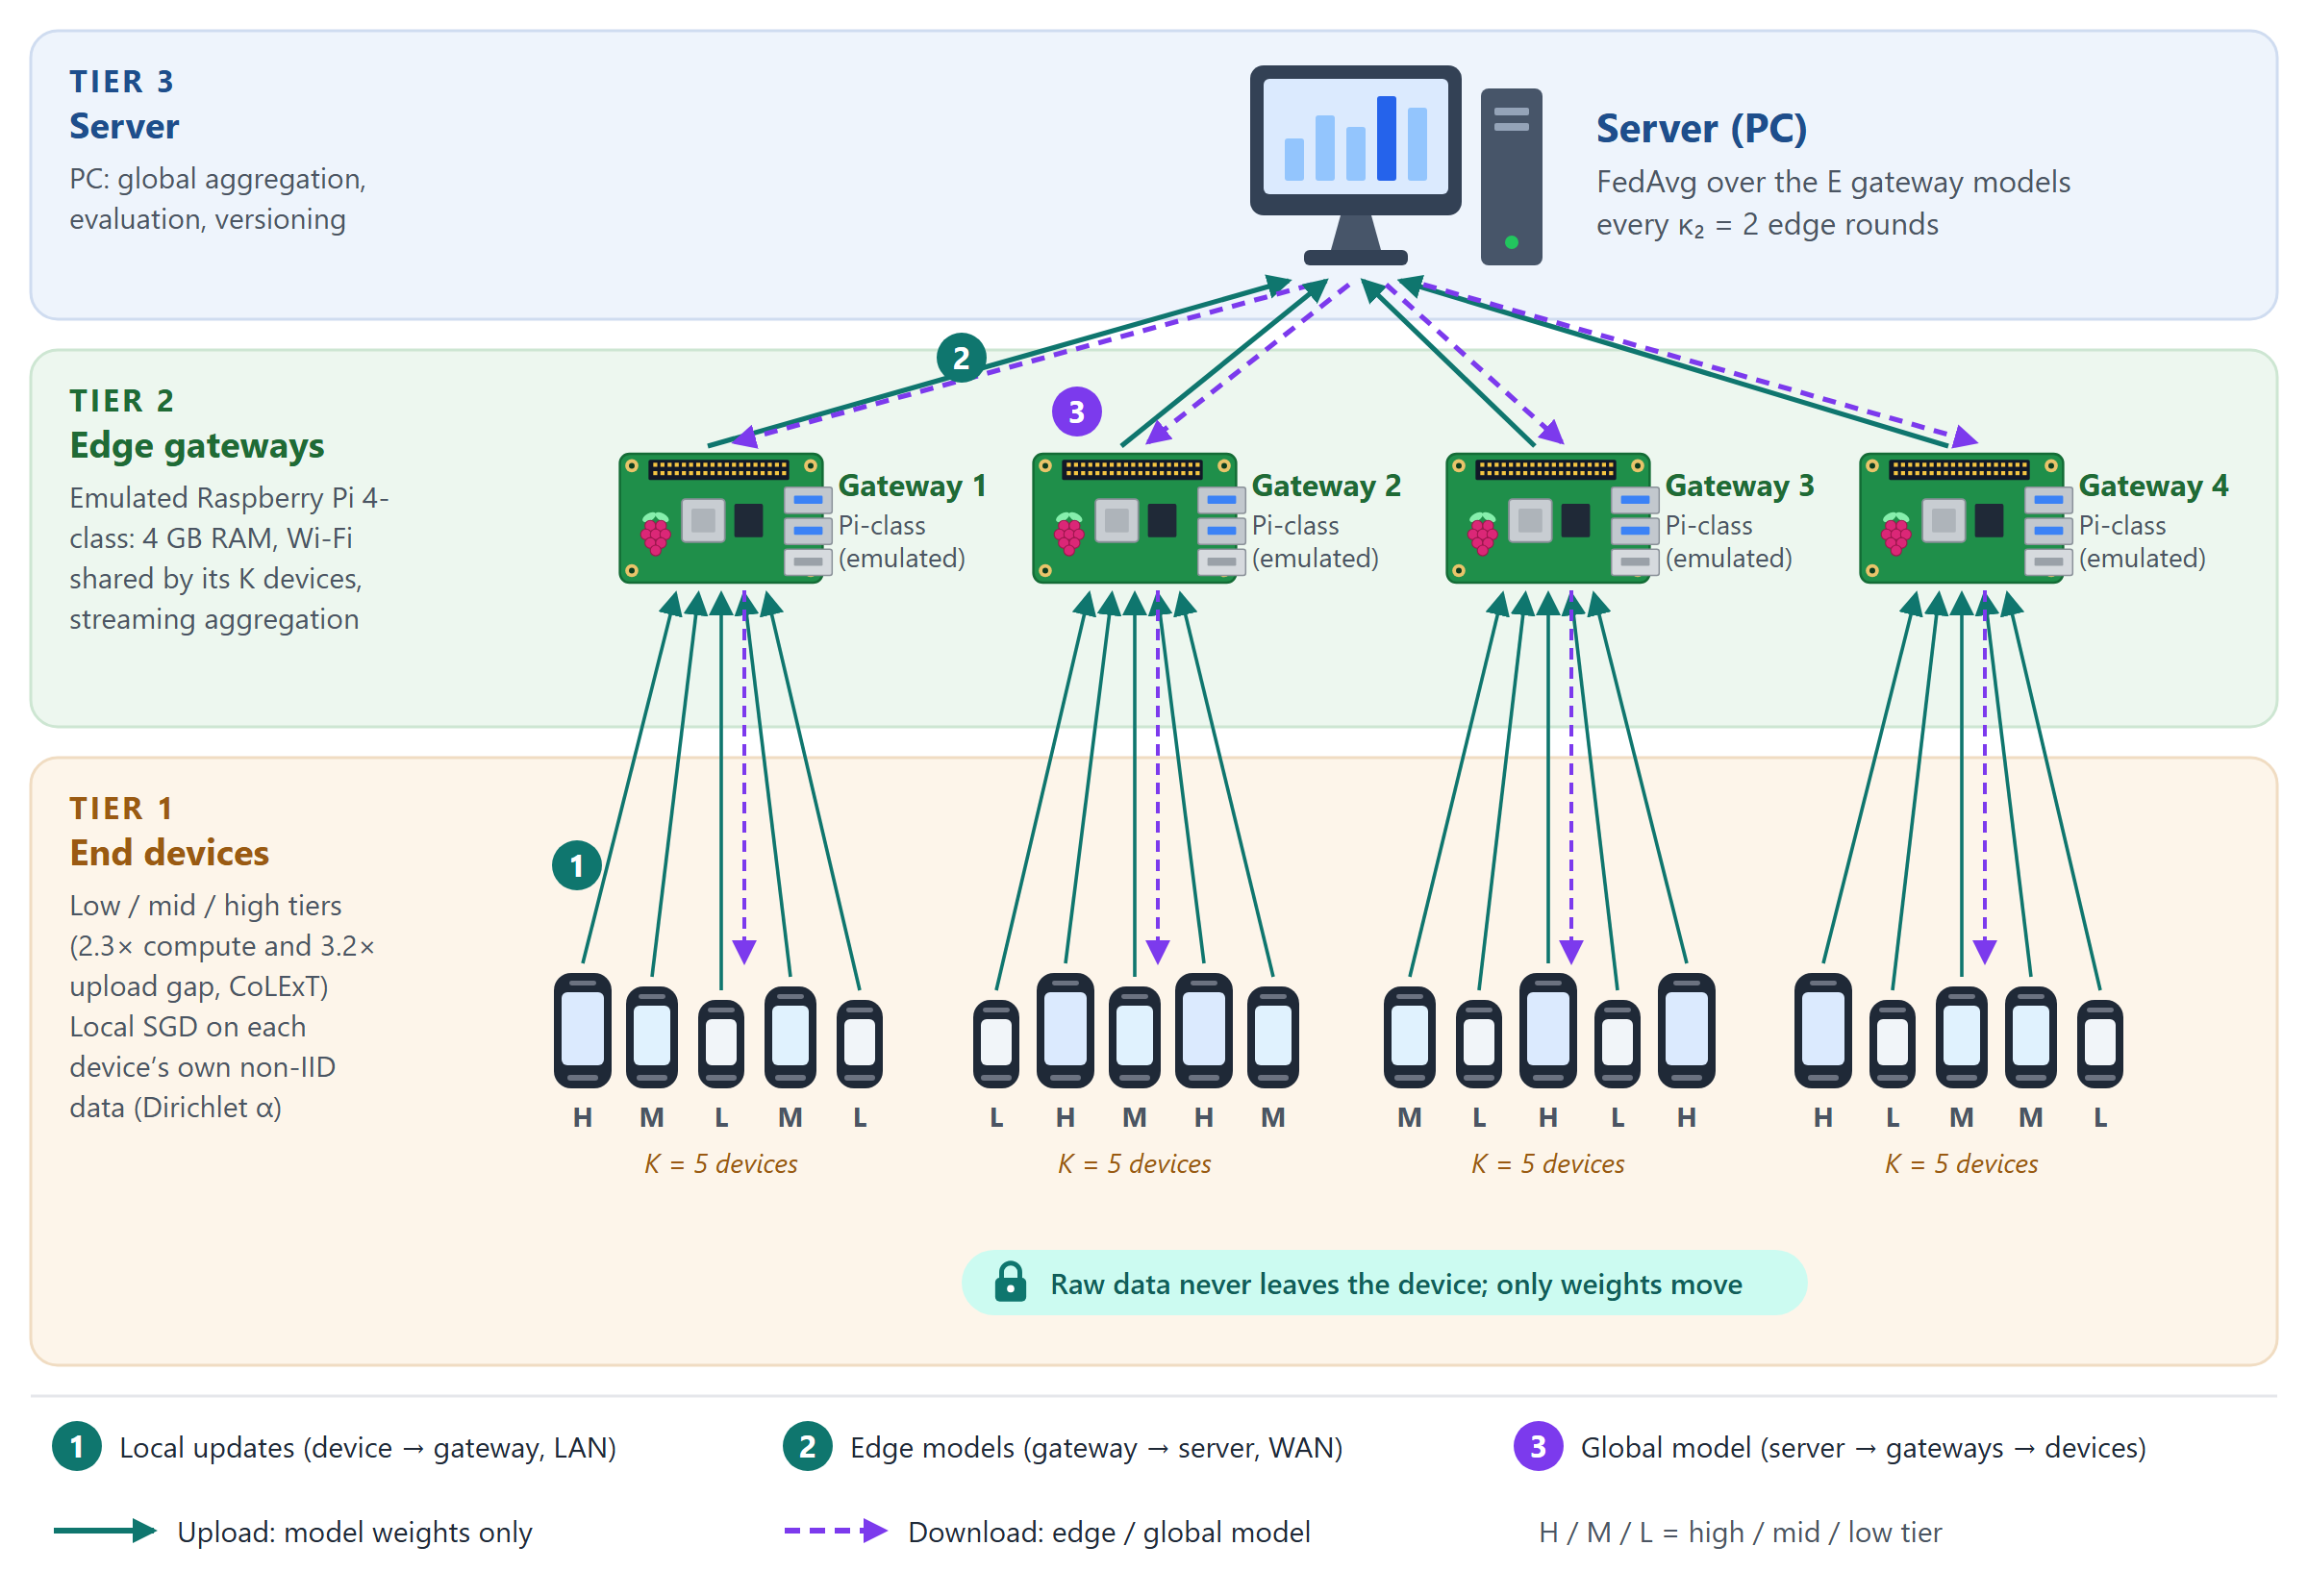
\includegraphics[width=\columnwidth]{figures/fig1_architecture.png}}{\figpending{figures/fig1\_architecture.png}}
\caption{Three-tier architecture. Heterogeneous devices (low, mid and high tier) train locally; $E$ emulated Raspberry Pi-class gateways aggregate the updates of their devices; the server combines the gateway models and returns the global model through the gateways. Only model weights are exchanged.}
\label{fig:arch}
\end{figure}

% ---------------------------------------------------------------------
\section{Related Work}
\label{sec:related}

We reviewed recent work (mainly 2024--2026) in four strands: hierarchical aggregation, system and model heterogeneity, real-hardware testbeds and hierarchical prototypes, and the privacy of shared weights. Papers were selected from peer-reviewed venues and checked against their publisher or arXiv records. Table~\ref{tab:lit} summarises the most relevant studies.

\begin{table*}[t]
\centering
\caption{Summary of related work on federated learning with heterogeneous edge devices}
\label{tab:lit}
\footnotesize
\renewcommand{\arraystretch}{1.12}
\begin{tabularx}{\textwidth}{@{}p{2.6cm}YYY@{}}
\toprule
\textbf{Work} & \textbf{Approach} & \textbf{Setup (data; scale)} & \textbf{Limitation for our setting} \\
\midrule
\multicolumn{4}{@{}l}{\textit{A. Hierarchical (client--edge--cloud) aggregation and non-IID data}} \\
FedAda~\cite{luo2024}, TSC 2024 & Client- and edge-level aggregation frequencies set from a convergence bound & Fashion-MNIST, CIFAR-10; Docker, 1 cloud, 4 edges, 20 clients & Simulation only; synthetic heterogeneity; capable edges \\
FedUC~\cite{ma2024feduc}, TMC 2024 & Clustering of non-IID workers to edge aggregators from convergence bounds & MNIST, CIFAR-10; 100 workers, 16 aggregators & Analytic wireless model; no hardware or energy \\
MTGC~\cite{fang2024mtgc}, NeurIPS 2024 & Two-level gradient correction for client and group drift & EMNIST, Fashion-MNIST, CIFAR-10/100; 100 clients, 10 groups, $\alpha=0.1$ & Ignores system heterogeneity; stateful clients fragile under dropout \\
ESPerHFL~\cite{ma2024esper}, JCC 2024 & Edge-level personalisation; similarity-weighted cloud aggregation & MNIST, Fashion-MNIST, CIFAR-10; 50 clients, 10 edges & About 4$\times$ FedAvg traffic; fixed client--edge mapping; no dropouts \\
\midrule
\multicolumn{4}{@{}l}{\textit{B. System and model heterogeneity}} \\
FedCompass~\cite{li2024fedcompass}, ICLR 2024 & Speed-aware number of local steps so client groups finish together & MNIST, CIFAR-10, Fed-IXI, Fed-ISIC2019; 5--20 clients & Flat, cross-silo; stable simulated speeds \\
FIARSE~\cite{wu2024fiarse}, NeurIPS 2024 & Importance-aware submodels for weak clients & CIFAR-10/100, AGNews; 100--200 clients & Unstructured sparsity poorly supported on mobile; simulation only \\
HAF-Edge~\cite{gao2024}, ICSOC 2024 & Architecture-grouped edges; distance-weighted edge aggregation & MNIST, Fashion-MNIST; up to 5 edges $\times$ 11 clients & Toy dense networks; no system costs \\
\midrule
\multicolumn{4}{@{}l}{\textit{C. Real-hardware testbeds and hierarchical prototypes}} \\
FedConv~\cite{shen2024fedconv}, MobiSys 2024 & Server-side convolutional compression into client submodels & MNIST, CIFAR-10, CINIC-10 and sensing sets; 20 real clients incl.\ Raspberry Pi 4 & Flat; Pi only a client; Android excluded \\
CoLExT~\cite{bozic2024}, SEC 2024 & Flower testbed with CPU, memory, network and power monitoring & CIFAR-10, FEMNIST; 20 Android phones, 28 single-board computers & Flat topology; no Raspberry Pi \\
FLEdge~\cite{woisetschlager2024}, Middleware 2024 & Benchmark with network emulation, dropouts and server-side DP & FEMNIST, Shakespeare and others; Pi 4B, Jetson boards & Star topology; no phones \\
Flotilla~\cite{banerjee2025}, JPDC 2025 & Fault-tolerant modular FL framework & EMNIST, CIFAR-10/100; 46 Pis, 12 Jetsons, up to 1,080 containers & Flat; hierarchy left to future work \\
FedCH~\cite{wang2023fedch}, TMC 2023 & Capacity-based clusters with header aggregation; asynchronous global step & MNIST, CIFAR-10; 20 Jetson TX2 boards & Aggregators are GPU-equipped boards \\
Qiu et al.~\cite{qiu2025}, FI 2025 & Sliding-window asynchronous edge aggregation; Salsa20 encryption & 4 Pi clients, 2 PC edges, 1 PC cloud; up to 20 emulated devices & Edges are PCs; heterogeneity mostly injected delay \\
\midrule
\multicolumn{4}{@{}l}{\textit{D. Privacy of shared weights}} \\
LOKI~\cite{zhao2024loki}, S\&P 2024 & Malicious-server reconstruction despite FedAvg and secure aggregation & MNIST, CIFAR-100, Tiny ImageNet; hundreds of clients & Active, architecture-modifying attacker \\
\bottomrule
\end{tabularx}
\end{table*}

\subsection{Hierarchical Aggregation and Non-IID Data}
The client--edge--cloud model of Liu \textit{et al.}~\cite{liu2020} has grown into a family of methods that tune \emph{how often} and \emph{among whom} aggregation happens: FedAda~\cite{luo2024} and AHFLP~\cite{su2025} set aggregation frequencies from convergence bounds, FedUC~\cite{ma2024feduc} assigns workers to edge aggregators, MTGC~\cite{fang2024mtgc} corrects client- and group-level drift, and ESPerHFL~\cite{ma2024esper} personalises at the edge. They show that a hierarchy can converge faster and communicate less than flat FL, but they are evaluated in simulation with sampled compute times or analytic channel models, and assume powerful, always-available edge servers.

\subsection{System and Model Heterogeneity}
FedCompass~\cite{li2024fedcompass} gives each client a number of local steps matched to its measured speed, avoiding both waiting for stragglers and the staleness of fully asynchronous FL; the idea maps directly onto a gateway that profiles its devices. FIARSE~\cite{wu2024fiarse} and HAF-Edge~\cite{gao2024} instead give weaker clients smaller models, and FedProx~\cite{li2020fedprox} is the standard way to tolerate variable local work on non-IID data. Client speeds in these works are simulated and assumed stable, whereas phones throttle and change load, so we use simple, measurable mechanisms (adaptive workload, deadlines, FedProx) rather than submodel schemes.

\subsection{Testbeds and Hierarchical Prototypes}
CoLExT~\cite{bozic2024} provides the most realistic phone evidence, quantifying straggler effects across eight Android models, but it is flat. FLEdge~\cite{woisetschlager2024} and Flotilla~\cite{banerjee2025} measure Raspberry Pi behaviour (FLEdge reports memory bottlenecks that make embedded boards roughly four times slower, and accuracy losses when dropouts meet differential privacy), but neither has a hierarchy. FedConv~\cite{shen2024fedconv} uses Raspberry Pi 4 clients but excludes Android because of integration obstacles with Flower~\cite{beutel2020flower}. The few physical hierarchies, FedCH~\cite{wang2023fedch} (20 Jetson TX2 boards with cluster headers) and Qiu \textit{et al.}~\cite{qiu2025} (four Pi clients under PC edge nodes), use GPU boards or PCs as aggregators. Across all of these systems the Raspberry Pi is a client, never the aggregator.

\subsection{Privacy of Shared Weights}
Sharing weights instead of data is necessary but not sufficient for privacy. LOKI~\cite{zhao2024loki} shows that a malicious server can reconstruct most training samples even under FedAvg and secure aggregation, while a systematisation of gradient-leakage attacks~\cite{du2025sok} finds that passive reconstruction becomes much harder with multiple local epochs and realistic batch sizes. Differential privacy (DP)~\cite{abadi2016}, \cite{mcmahan2018dp} and secure aggregation~\cite{bonawitz2017} provide formal protection at a cost in accuracy or computation. This work treats ``weights only'' as the baseline guarantee and leaves edge-level DP to future work.

\subsection{Device Counts in the Base Papers}
Table~\ref{tab:counts} lists the populations used by the hierarchical base papers. Fashion-MNIST is the most widely shared dataset (four of the five papers), and the configurations range from 4 to 16 edges and from 20 to 100 clients. Rather than choosing an arbitrary population, we fix our main configuration to FedAda's 4 gateways $\times$ 5 clients for direct comparability, and add a sweep that gradually increases the clients per gateway ($K = 5 \rightarrow 10 \rightarrow 25$) and the number of gateways ($E = 2 \rightarrow 4 \rightarrow 10$), reaching the 100-client scale of MTGC and FedUC. As in these papers, the dataset is fixed, so adding clients reduces the data per client.

\begin{table}[t]
\centering
\caption{Populations in the hierarchical base papers and in this work}
\label{tab:counts}
\footnotesize
\setlength{\tabcolsep}{2.5pt}
\begin{tabular}{@{}lccl@{}}
\toprule
\textbf{Paper} & \textbf{Edges} & \textbf{Clients} & \textbf{Datasets} \\
\midrule
FedAda~\cite{luo2024} & 4 & 20 & FMNIST, CIFAR-10 \\
HAF-Edge~\cite{gao2024} & $\le 5$ & 11 per edge & MNIST, FMNIST \\
ESPerHFL~\cite{ma2024esper} & 10 & 50 & MNIST, FMNIST, CIFAR-10 \\
MTGC~\cite{fang2024mtgc} & 10 & 100 & EMNIST, FMNIST, CIFAR-10/100 \\
FedUC~\cite{ma2024feduc} & 16 & 100 & MNIST, CIFAR-10 \\
\midrule
This work (main) & 4 & 20 & FMNIST \\
This work (sweep) & 2--10 & 10--100 & FMNIST \\
\bottomrule
\end{tabular}
\end{table}

\subsection{Research Gap}
Algorithmic HFL papers are evaluated in simulation with capable edge servers and synthetic device speeds; hardware testbeds are flat and use the Raspberry Pi only as a client; and the few hierarchical prototypes use GPU boards or PCs as aggregators. Among the works we reviewed, none treats the edge aggregator itself as a resource-constrained device and quantifies how its limits interact with heterogeneous clients and with heterogeneity-aware mechanisms as the number of clients per gateway grows. This work addresses that question in a reproducible emulation whose device and gateway parameters are taken from published measurements and from measurements of our own phones. We do not claim results on physical gateways; validating the findings on real Raspberry Pi hardware is future work.

% ---------------------------------------------------------------------
\section{Problem Statement and Research Questions}
\label{sec:problem}

Given $N$ devices with heterogeneous speeds and non-IID data, grouped under $E$ resource-constrained gateways, the goal is to train an accurate global model while exchanging only model weights, and to quantify how statistical and system heterogeneity, the edge tier, heterogeneity-aware mechanisms and the number of devices per gateway affect accuracy, fairness across devices, training time and communication. We address four research questions:

\begin{description}
\item[RQ1] How much do statistical and system heterogeneity degrade accuracy and convergence relative to centralised training?
\item[RQ2] Does a Pi-class edge tier reduce server-side communication and round latency compared with flat FL, without loss of accuracy?
\item[RQ3] Do FedProx, deadline-based partial aggregation and adaptive local workload improve accuracy, worst-device accuracy and time-to-accuracy over FedAvg?
\item[RQ4] How do accuracy, round time and gateway load change as the number of devices per gateway and the number of gateways grow?
\end{description}

\noindent We test two hypotheses:

\begin{description}
\item[H1] Under Dirichlet label skew and mixed device tiers, hierarchical FedProx with deadline-based aggregation and adaptive local workload achieves higher accuracy, higher 10th-percentile client accuracy and shorter time-to-target than hierarchical FedAvg.
\item[H2] The hierarchical configuration transmits fewer bytes to the server per unit of accuracy than flat FL, while gateway aggregation time and memory remain within Pi-class limits.
\end{description}

% ---------------------------------------------------------------------
\section{Methodology}
\label{sec:method}

\subsection{System Model}
The system has three tiers (Fig.~\ref{fig:arch}). Tier~1 consists of $N$ devices drawn from three performance tiers (low, mid, high), matching the budget, mid-range and flagship phones of the original design. Tier~2 consists of $E$ Raspberry Pi-class gateways; gateway $e$ serves a fixed set $\mathcal{C}_e$ of $K = N/E$ devices assigned uniformly at random. Tier~3 is a server that aggregates gateway models, evaluates and versions the global model, and returns it through the gateways. Client $k$ holds $n_k$ training samples; gateway $e$ holds $n_e = \sum_{k \in \mathcal{C}_e} n_k$ and the total is $n = \sum_e n_e$. The model has $\wsize$ bytes.

Training follows HierFAVG~\cite{liu2020}. In each \emph{edge round}, every device trains locally, and each gateway aggregates the updates it receives into an edge model. Every $\kappa_2$ edge rounds, a \emph{global round} ends: gateways send their edge models to the server, which aggregates them and returns the global model. With sample-weighted FedAvg~\cite{mcmahan2017} at both tiers,
\begin{equation}
w_e = \frac{\sum_{k \in \mathcal{S}_e} n_k w_k}{\sum_{k \in \mathcal{S}_e} n_k}, \qquad
w = \sum_{e=1}^{E} \frac{n_e}{n} w_e ,
\label{eq:agg}
\end{equation}
where $\mathcal{S}_e \subseteq \mathcal{C}_e$ is the set of updates accepted in that edge round. If no update of a gateway is accepted, the gateway keeps its previous edge model.

\subsection{Data and Partitioning}
We use Fashion-MNIST~\cite{xiao2017fmnist}: 60{,}000 training and 10{,}000 test greyscale images of $28\times 28$ pixels in ten balanced clothing classes, normalised with mean 0.2860 and standard deviation 0.3530. It is shared by four of our five hierarchical base papers (Table~\ref{tab:counts}). Statistical heterogeneity is controlled with Dirichlet label skew~\cite{hsu2019}: for each class, its samples are split across the $N$ clients with proportions drawn from $\mathrm{Dir}(\alpha)$, where a client that already holds its fair share receives no more of the class, resampling until every client holds at least 10 samples (the NIID-Bench procedure). We use $\alpha \in \{0.1, 0.5, 1.0\}$ (smaller is more skewed) and an IID split as a sanity check. Clients train on all of their samples; global accuracy is measured on the official test set.

\subsection{Model and Local Training}
The model is a compact convolutional network: Conv($1\!\rightarrow\!16$, $3\times3$) -- ReLU -- MaxPool(2) -- Conv($16\!\rightarrow\!32$, $3\times3$) -- ReLU -- MaxPool(2) -- FC($1568\!\rightarrow\!48$) -- ReLU -- FC($48\!\rightarrow\!10$). It has 80{,}602 parameters, so $\wsize = 322{,}408$~bytes (315~KiB) in float32, which meets the proposal's target of fewer than 100k parameters and under 1~MB. It has no batch normalisation, so weights are plain tensors and averaging is exact. Each device runs one local epoch per edge round with SGD (learning rate 0.05, batch size 32), i.e.\ $\tau_k^{\mathrm{full}} = \lceil n_k/32 \rceil$ steps, minimising
\begin{equation}
\min_{w}\; F_k(w) + \frac{\mu}{2}\,\| w - w_e^{t} \|^2 ,
\label{eq:prox}
\end{equation}
where $F_k$ is the cross-entropy loss on the device's data and $w_e^{t}$ is the edge model received at the start of the round. FedAvg uses $\mu = 0$ and FedProx~\cite{li2020fedprox} uses $\mu = 0.01$.

\subsection{Device and Gateway Profiles}
Table~\ref{tab:params} lists every system parameter with its source. Device speed ratios are taken from measurements on real phones: the low/high compute ratio of 2.3$\times$ and the high/low upload ratio of 3.2$\times$ come from CoLExT~\cite{bozic2024}. The mid tier is set from measurements of our own phones: we ran the same network in TensorFlow.js~\cite{smilkov2019tfjs} (CPU backend) in the browser of a low-end and a mid-range phone and measured the median time per training step with batch size 32. \todo{phone models and measured ms/step for both phones; resulting mid/low ratio. If not measured, state that the mid tier uses the geometric mean of the low and high tiers (1.52$\times$ the high tier).} Because the browser runtime differs from native on-device training, only the ratio between phones is used. The absolute scale ($t_{\mathrm{high}} = 20$~ms per step) is an assumption; it affects the balance between computation and communication time, not the ranking of methods. The gateway profile follows a Raspberry Pi~4 Model B with 4~GB RAM~\cite{rpi4brief}.

\begin{table}[t]
\centering
\caption{Device, network and gateway parameters (A = assumption)}
\label{tab:params}
\footnotesize
\renewcommand{\arraystretch}{1.1}
\begin{tabularx}{\columnwidth}{@{}p{2.45cm}p{2.25cm}Y@{}}
\toprule
\textbf{Parameter} & \textbf{Value} & \textbf{Source} \\
\midrule
Device tiers & low, mid, high & Budget, mid-range and flagship phones of the original design \\
Step time, high tier & $t_{\mathrm{high}} = 20$ ms & A (scale only) \\
Low/high compute ratio & 2.3$\times$ & CoLExT~\cite{bozic2024} \\
Mid tier & \todo{measured} ratio & Own phones; else A: 1.52$\times$ (geometric mean) \\
Per-round speed jitter & $\mathrm{LogN}(0, 0.2^2)$ & A: throttling and background load \\
Phone WAN uplink (flat FL) & 20 / 12 / 6.25 Mbit/s (high/mid/low) & High/low ratio 3.2$\times$ from CoLExT~\cite{bozic2024}; absolute values A \\
Gateway Wi-Fi LAN & 50 Mbit/s shared, $50/K$ per device & A: Pi~4 on-board 802.11ac \\
Gateway WAN uplink & $B_{\mathrm{gw}} = 20$ Mbit/s & A: broadband link \\
Gateway aggregation & $\delta = 5$ ms per update $+\;\wsize/\rho$, $\rho = 400$ MB/s & A: memory-bound weighted sum; embedded boards $\approx$4$\times$ slower~\cite{woisetschlager2024} \\
Gateway RAM & 4 GB & Raspberry Pi~4 Model B~\cite{rpi4brief} \\
Tier mixes & mixed: $\frac13$ each; mid: all mid; low-heavy: 60/30/10\% & Design choice \\
\bottomrule
\end{tabularx}
\end{table}

\subsection{Cost Model}
\label{sec:cost}
The simulator keeps a simulated clock that is independent of the real run time. Let $t_k$ be device $k$'s nominal time per step, $j_k \sim \mathrm{LogN}(0, 0.2^2)$ its jitter in the current round, $\tau_k$ its number of local steps, and $b_k^{\downarrow}, b_k^{\uparrow}$ its download and upload rates (LAN fair share $50/K$~Mbit/s in the hierarchy, tier-dependent WAN rates in flat FL). The device's finish time and communication time are
\begin{equation}
T_k = \underbrace{\frac{\wsize}{b_k^{\downarrow}} + \frac{\wsize}{b_k^{\uparrow}}}_{c_k} + \tau_k\, t_k\, j_k .
\label{eq:tk}
\end{equation}
A gateway that accepts $m$ updates spends $A_e = m\,(\delta + \wsize/\rho)$ aggregating them. Without a deadline, the gateway waits for all of its devices:
\begin{equation}
T_e = \max_{k \in \mathcal{C}_e} T_k + A_e .
\label{eq:sync}
\end{equation}
With a deadline $D$, only updates with $T_k \le D$ are accepted ($\mathcal{S}_e = \{k : T_k \le D\}$); the steps of late devices count as wasted computation, and
\begin{equation}
T_e = \begin{cases} D + A_e & \text{if } \mathcal{S}_e \neq \mathcal{C}_e,\\ \max_{k \in \mathcal{C}_e} T_k + A_e & \text{otherwise.} \end{cases}
\label{eq:deadline}
\end{equation}
The deadline is set once per run to the expected full-epoch finish time of the median device, $D = \operatorname{median}_k \big(c_k + \tau_k^{\mathrm{full}} t_k\big)$, so roughly half of the devices cannot complete a full epoch in time. Gateways run their edge rounds in parallel, and a global round ends when the slowest gateway has completed $\kappa_2 = 2$ edge rounds and uploaded its model over its WAN link:
\begin{equation}
T_{\mathrm{glob}} = \max_{e} \Big( \sum_{r=1}^{\kappa_2} T_e^{(r)} + \frac{\wsize}{B_{\mathrm{gw}}} \Big) + \frac{\wsize}{B_{\mathrm{gw}}} .
\label{eq:global}
\end{equation}
In flat FedAvg, all $N$ devices exchange weights directly with the server over their WAN links, so a round takes $T_{\mathrm{round}} = \max_k T_k$ with WAN rates; server-side aggregation on the PC is treated as free.

\textit{Communication.} In flat FL every round moves $2N\wsize$ bytes through the server. In the hierarchy, every edge round moves $2N\wsize$ bytes over the gateways' LANs, but only $2E\wsize$ bytes reach the server per global round. Over $R$ edge rounds the server traffic is therefore $2NR\wsize$ for flat FL and $2E(R/\kappa_2)\wsize$ for the hierarchy, a reduction by a factor of $K\kappa_2$ (10 in the main configuration: 773.8~MB versus 77.4~MB over 60 rounds). The measured question for RQ2 is whether this saving costs accuracy or time.

For scale, a high-tier device with the average 3{,}000 samples of the main configuration needs 94 steps (1.9~s) per epoch, while sending the model over its LAN share takes 0.26~s; computation therefore dominates the round time. Aggregating five updates takes the gateway about 29~ms.

\subsection{Heterogeneity-Aware Mechanisms}
\textit{Device profiling.} Each device reports its nominal time per step and link rate to its gateway, which stores the profile.

\textit{Deadline-based partial aggregation.} Instead of waiting for every device (Eq.~\ref{eq:sync}), the gateway aggregates the updates that arrive by the deadline $D$ and discards late ones (Eq.~\ref{eq:deadline}), so a straggler cannot stall its group.

\textit{Adaptive local workload.} Following FedCompass~\cite{li2024fedcompass}, the gateway gives each device the number of steps it can complete before the deadline. Planning with the nominal speed alone would leave about half of the slowed-down devices late, because the jitter $j_k$ has median 1; the gateway therefore plans for a slow round, inflating the profiled step time by the 90th percentile of the jitter, $\gamma = e^{z_{0.9}\sigma} \approx 1.29$:
\begin{equation}
\tau_k = \operatorname{clip}\!\left( \left\lfloor \frac{D - c_k}{\gamma\, t_k} \right\rfloor,\ \tau_{\min},\ \tau_k^{\mathrm{full}} \right), \quad \tau_{\min} = \lceil 0.1\,\tau_k^{\mathrm{full}} \rceil .
\label{eq:adaptive}
\end{equation}
Fast devices still train a full epoch, slow devices train fewer steps instead of being dropped, and only rounds slower than the 90th percentile make a planned device miss $D$.

\textit{Drift control.} FedProx (Eq.~\ref{eq:prox}) limits how far a device's model moves from the edge model, which matters when devices perform different amounts of local work.

\textit{Streaming aggregation at the gateway.} Instead of buffering all $K$ updates before averaging, the gateway keeps a running weighted mean: on receiving $w_k$ it sets $m \leftarrow m + n_k$ and $\bar{w} \leftarrow \bar{w} + \frac{n_k}{m}(w_k - \bar{w})$. The result equals Eq.~(\ref{eq:agg}), but the gateway holds only the accumulator and the incoming update, i.e.\ $2\wsize$ of memory regardless of $K$, instead of $K\wsize$. For our model the difference is small (0.64~MB versus 8.1~MB at $K = 25$), but it grows with model size: for ResNet-18~\cite{he2016resnet} (11{,}689{,}512 parameters, $\wsize = 46.8$~MB), a buffered gateway serving 100 devices would need 4.68~GB, more than the 4~GB (4.29~GB) of RAM of a Raspberry Pi~4, whereas streaming needs 93.5~MB.

Algorithm~\ref{alg:round} summarises one global round of the proposed scheme.

\begin{algorithm}[t]
\caption{One global round of the proposed scheme}
\label{alg:round}
\small
\begin{algorithmic}[1]
\Require global model $w$; gateways $e$ with device sets $\mathcal{C}_e$; profiles $(t_k, c_k)$; deadline $D$; $\kappa_2$; $\mu$
\ForAll{gateways $e$ \textbf{in parallel}}
  \State $w_e \gets w$
  \For{$r = 1, \dots, \kappa_2$}
    \State $\bar{w} \gets 0$; $m \gets 0$
    \ForAll{devices $k \in \mathcal{C}_e$}
      \State $\tau_k \gets$ Eq.~(\ref{eq:adaptive}); sample $j_k$; compute $T_k$ (Eq.~\ref{eq:tk})
      \If{$T_k \le D$}
        \State $w_k \gets \textsc{LocalSGD}(w_e, \tau_k, \mu)$ \Comment{Eq.~(\ref{eq:prox})}
        \State $m \gets m + n_k$; $\bar{w} \gets \bar{w} + \frac{n_k}{m}(w_k - \bar{w})$
      \EndIf
    \EndFor
    \If{$m > 0$}
      \State $w_e \gets \bar{w}$
    \EndIf
    \State advance the gateway clock by $T_e^{(r)}$ (Eq.~\ref{eq:deadline})
  \EndFor
  \State send $w_e$ to the server
\EndFor
\State $w \gets \sum_e \frac{n_e}{n} w_e$; advance the global clock by $T_{\mathrm{glob}}$ (Eq.~\ref{eq:global})
\State \Return $w$
\end{algorithmic}
\end{algorithm}

\subsection{Methods Compared}
Table~\ref{tab:methods} lists the methods. The first two are the upper and lower bounds of the proposal; flat and hierarchical FedAvg are the baselines; the last three add the mechanisms one at a time, so that the final configuration (the proposed scheme) forms an ablation. All federated methods get the same budget of $R = 60$ edge rounds (flat FedAvg: 60 rounds), i.e.\ the same maximum local computation.

\begin{table}[t]
\centering
\caption{Methods compared}
\label{tab:methods}
\footnotesize
\setlength{\tabcolsep}{2.5pt}
\begin{tabular}{@{}llccc@{}}
\toprule
\textbf{Method} & \textbf{Topology} & \textbf{FedProx} & \textbf{Deadline} & \textbf{Adapt.\ $\tau$} \\
\midrule
Centralised & pooled data (upper bound) & -- & -- & -- \\
Local-only & per device (lower bound) & -- & -- & -- \\
Flat FedAvg & device $\rightarrow$ server & no & no & no \\
H-FedAvg & device $\rightarrow$ GW $\rightarrow$ server & no & no & no \\
H-FedProx & hierarchical & yes & no & no \\
H-FedProx+DL & hierarchical & yes & yes & no \\
Proposed & hierarchical & yes & yes & yes \\
\bottomrule
\end{tabular}
\end{table}

\subsection{Implementation}
The proposal planned to orchestrate training with Flower~\cite{beutel2020flower}. As anticipated in its risk analysis, Flower provides no native multi-level aggregation, and its simulation engine measures real run time on the host rather than the time a low-end device or a Pi-class gateway would take. We therefore implemented the hierarchy directly in PyTorch~\cite{paszke2019pytorch}, following the HierFAVG structure~\cite{liu2020} and the simulated evaluation setups of the base papers~\cite{luo2024}, \cite{fang2024mtgc}. Devices are trained one after another in a single process with all data resident on the GPU; the simulated clock and byte counters follow Section~\ref{sec:cost} and do not depend on how fast the host runs. Experiments ran on a laptop with an NVIDIA GeForce RTX 5060 Laptop GPU (8~GB), Python 3.13 and PyTorch 2.8. As a correctness check, flat and hierarchical FedAvg on an IID split should approach the centralised accuracy.

\subsection{Privacy Model}
Raw data never leaves a device; only weights, sample counts and coarse profiles are transmitted. Because shared weights can still leak information~\cite{zhao2024loki}, \cite{du2025sok}, edge-level differential privacy at the gateway (clipping each update and adding calibrated Gaussian noise before forwarding~\cite{mcmahan2018dp}) remains the stretch goal of the proposal and is left to future work.

% ---------------------------------------------------------------------
\section{Experimental Setup}
\label{sec:setup}

\textit{Experiment groups.} Three groups of experiments answer the research questions:
\begin{itemize}
\item \textbf{G1 (main; RQ1--RQ3):} $E = 4$, $K = 5$ ($N = 20$), mixed tiers, $\alpha \in \{0.1, 0.5, 1.0\}$, all methods, seeds $\{0, 1, 2\}$, plus flat and hierarchical FedAvg on an IID split.
\item \textbf{G2 (system heterogeneity; RQ1):} $\alpha = 0.5$, tier mixes all-mid and low-heavy, methods H-FedAvg, H-FedProx+DL and Proposed, seeds $\{0, 1, 2\}$.
\item \textbf{G3 (scaling; RQ4):} $\alpha = 0.5$, mixed tiers, $(E, K) \in \{(4,10), (4,25), (2,5), (10,5)\}$ together with $(4,5)$ from G1, methods Flat FedAvg, H-FedAvg and Proposed, seeds $\{0, 1\}$.
\end{itemize}
A seed fixes the data partition, the device-to-gateway assignment, the tier assignment, the jitter and the model initialisation.

\textit{Metrics.} The primary metric is top-1 accuracy of the global model on the official test set, the metric reported by the base papers. To measure how well the shared model serves each skewed device, we compute a per-client accuracy under the client's own label distribution, $\mathrm{acc}_k = \sum_{c} p_{k,c}\, \mathrm{acc}_c$, where $\mathrm{acc}_c$ is the global model's accuracy on test class $c$ and $p_{k,c}$ is the fraction of client $k$'s samples in class $c$. This is exact (no sampling noise from small local test sets). We report the \emph{10th-percentile client accuracy} across clients as the worst-device metric; for the local-only baseline, each client's own model is used. Table~\ref{tab:rqmetrics} maps each research question to its experiments and metrics. Evaluation happens at every global round (every round for flat FedAvg). Results are reported as mean $\pm$ standard deviation over seeds, and differences between methods are checked with paired t-tests over seeds and $\alpha$ settings.

\begin{table}[t]
\centering
\caption{Research questions, experiments and metrics}
\label{tab:rqmetrics}
\footnotesize
\renewcommand{\arraystretch}{1.1}
\begin{tabularx}{\columnwidth}{@{}p{0.75cm}p{2.5cm}Y@{}}
\toprule
\textbf{RQ} & \textbf{Experiment} & \textbf{Metrics that answer it} \\
\midrule
RQ1 & $\alpha$ sweep and tier mixes (G1, G2) & Accuracy gap to centralised; rounds and simulated time to target accuracy \\
RQ2 & Flat vs.\ hierarchical FedAvg, same computation (G1) & Bytes to and from the server; simulated round time; final accuracy \\
RQ3 & Ablation H-FedAvg $\rightarrow$ Proposed (G1) & Final accuracy; 10th-percentile client accuracy; time to target; dropped updates; wasted steps \\
RQ4 & $K$ and $E$ sweeps (G3) & Final accuracy; simulated round time; gateway aggregation time and memory; bytes \\
\bottomrule
\end{tabularx}
\end{table}

% ---------------------------------------------------------------------
\section{Results}
\label{sec:results}

Table~\ref{tab:main} summarises the main configuration and Table~\ref{tab:scaling} the scaling sweep. \todo{state the target accuracy used for time-to-target (e.g., 90\% of the centralised final accuracy) and the total number of runs.}

\begin{table*}[t]
\centering
\caption{Main configuration ($E = 4$, $K = 5$, mixed tiers): final accuracy, 10th-percentile client accuracy, time to target and server traffic (mean $\pm$ std over three seeds)}
\label{tab:main}
\footnotesize
% generated by analyze.py -- do not edit
\begin{tabular}{l cc cc cc cccc}
\toprule
 & \multicolumn{2}{c}{$\alpha = 0.1$} & \multicolumn{2}{c}{$\alpha = 0.5$} & \multicolumn{2}{c}{$\alpha = 1.0$} & \multicolumn{4}{c}{$\alpha = 0.5$} \\
\cmidrule(lr){2-3}\cmidrule(lr){4-5}\cmidrule(lr){6-7}\cmidrule(lr){8-11}
Method & Acc & P10 & Acc & P10 & Acc & P10 & $T_{\mathrm{tgt}}$ (s) & $R_{\mathrm{tgt}}$ & Server (MB) & Dropped (\%) \\
\midrule
Centralised & 90.9$\pm$0.3 & 84.5$\pm$1.7 & 90.6$\pm$0.6 & 86.5$\pm$1.8 & 90.8$\pm$0.4 & 87.7$\pm$1.6 & -- & -- & -- & -- \\
Local-only & 33.4$\pm$2.1 & 92.9$\pm$1.9 & 62.6$\pm$1.0 & 86.1$\pm$0.1 & 71.0$\pm$1.9 & 85.4$\pm$0.8 & -- & -- & -- & -- \\
\midrule
Flat FedAvg & \textbf{85.9$\pm$0.9} & \textbf{74.7$\pm$6.8} & 88.6$\pm$0.5 & 82.6$\pm$2.8 & 89.4$\pm$0.3 & \textbf{85.6$\pm$1.3} & 69 & 9 & 773.8 & 0.0 \\
H-FedAvg & 85.7$\pm$1.5 & 73.7$\pm$9.8 & 88.6$\pm$0.7 & 83.4$\pm$3.1 & \textbf{89.4$\pm$0.1} & 85.1$\pm$0.3 & 69 & 10 & 77.4 & 0.0 \\
H-FedProx & 85.7$\pm$1.5 & 73.5$\pm$9.4 & \textbf{88.7$\pm$0.7} & \textbf{83.5$\pm$3.1} & 89.4$\pm$0.2 & 85.0$\pm$0.5 & 69 & 10 & 77.4 & 0.0 \\
H-FedProx+DL & 80.7$\pm$3.5 & 62.2$\pm$18.9 & 87.9$\pm$0.7 & 82.3$\pm$2.4 & 88.9$\pm$0.5 & 85.0$\pm$2.0 & 52 & 14 & 77.4 & 45.6 \\
Proposed & 83.2$\pm$1.0 & 69.6$\pm$11.9 & 87.6$\pm$0.5 & 81.4$\pm$3.1 & 88.9$\pm$0.3 & 85.3$\pm$1.3 & 48 & 13 & 77.4 & 5.8 \\
\bottomrule
\end{tabular}

\end{table*}

\subsection{RQ1: Cost of Statistical and System Heterogeneity}
Fig.~\ref{fig:rq1} shows final accuracy across label-skew levels and tier mixes. \todo{Report the accuracy gap between centralised training and each federated method for $\alpha = 0.1, 0.5, 1.0$ and IID, and how the gap and the rounds/simulated time to target change when the tier mix goes from all-mid to mixed to low-heavy (G2). Confirm the IID sanity check (flat and hierarchical FedAvg close to centralised).}

\begin{figure}[t]
\centering
\IfFileExists{figures/fig_rq1_heterogeneity.pdf}{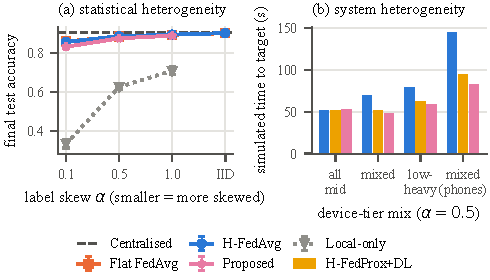
\includegraphics[width=\columnwidth]{figures/fig_rq1_heterogeneity.pdf}}{\figpending{figures/fig\_rq1\_heterogeneity.pdf}}
\caption{RQ1: final test accuracy versus label skew $\alpha$ and device-tier mix, relative to the centralised upper bound and the local-only lower bound.}
\label{fig:rq1}
\end{figure}

\subsection{RQ2: Value of the Pi-Class Edge Tier}
Fig.~\ref{fig:rq2} compares flat and hierarchical FedAvg at equal local computation. \todo{Compare flat FedAvg and H-FedAvg: accuracy versus bytes through the server and versus simulated time; report the measured server-traffic reduction (expected factor $K\kappa_2 = 10$) and whether final accuracy differs significantly. Report bytes per accuracy point (H2).}

\begin{figure}[t]
\centering
\IfFileExists{figures/fig_rq2_comm.pdf}{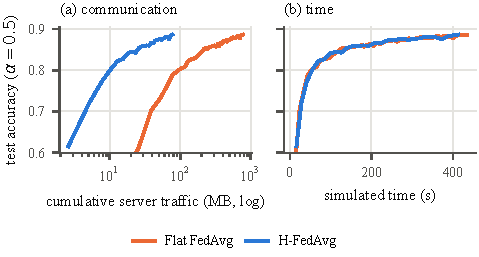
\includegraphics[width=\columnwidth]{figures/fig_rq2_comm.pdf}}{\figpending{figures/fig\_rq2\_comm.pdf}}
\caption{RQ2: test accuracy of flat and hierarchical FedAvg versus cumulative bytes through the server (left) and simulated time (right).}
\label{fig:rq2}
\end{figure}

\subsection{RQ3: Contribution of the Heterogeneity-Aware Mechanisms}
Fig.~\ref{fig:rq3} and Table~\ref{tab:main} show the ablation. \todo{Walk through the ablation H-FedAvg $\rightarrow$ H-FedProx $\rightarrow$ H-FedProx+DL $\rightarrow$ Proposed: final accuracy, 10th-percentile client accuracy, time to target, fraction of dropped updates and wasted steps. Note which step contributes most and whether the deadline alone hurts fairness under strong skew. Report paired t-test p-values (H1).}

\begin{figure}[t]
\centering
\IfFileExists{figures/fig_rq3_ablation.pdf}{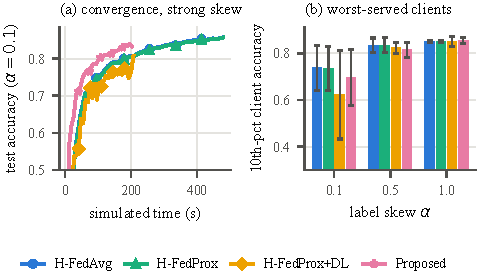
\includegraphics[width=\columnwidth]{figures/fig_rq3_ablation.pdf}}{\figpending{figures/fig\_rq3\_ablation.pdf}}
\caption{RQ3: ablation of the heterogeneity-aware mechanisms: test accuracy versus simulated time, and 10th-percentile client accuracy.}
\label{fig:rq3}
\end{figure}

\subsection{RQ4: Scaling with Devices per Gateway and Gateways}
Fig.~\ref{fig:rq4} and Table~\ref{tab:scaling} report the scaling sweep. \todo{Report how final accuracy, simulated round time, gateway aggregation time and memory, and server/edge bytes change for $K = 5, 10, 25$ ($E = 4$) and $E = 2, 4, 10$ ($K = 5$). Identify which resource (LAN share, aggregation time, waiting for stragglers) grows fastest and whether a Pi-class gateway becomes the bottleneck within the tested range.}

\begin{table}[t]
\centering
\caption{Scaling sweep ($\alpha = 0.5$, mixed tiers; mean over two seeds)}
\label{tab:scaling}
\footnotesize
% generated by analyze.py -- do not edit
\setlength{\tabcolsep}{3pt}
\begin{tabular}{lr ccc cc r}
\toprule
 & & \multicolumn{3}{c}{Accuracy (\%)} & \multicolumn{2}{c}{$\bar T_r$ (s)} & \\
\cmidrule(lr){3-5}\cmidrule(lr){6-7}
$E{\times}K$ & $N$ & Flat & H-Avg & Prop. & H-Avg & Prop. & $A_e$ (ms) \\
\midrule
4$\times$5 & 20 & 88.8 & 89.0 & 87.7 & 7.28 & 3.67 & 27 \\
4$\times$10 & 40 & 87.3 & 87.8 & 87.0 & 4.61 & 2.66 & 54 \\
4$\times$25 & 100 & 84.9 & 84.6 & 82.9 & 4.68 & 3.43 & 139 \\
2$\times$5 & 10 & 90.3 & 90.4 & 89.7 & 11.73 & 6.40 & 27 \\
10$\times$5 & 50 & 87.3 & 87.2 & 86.2 & 3.55 & 1.77 & 27 \\
\bottomrule
\end{tabular}

\end{table}

\begin{figure}[t]
\centering
\IfFileExists{figures/fig_rq4_scaling.pdf}{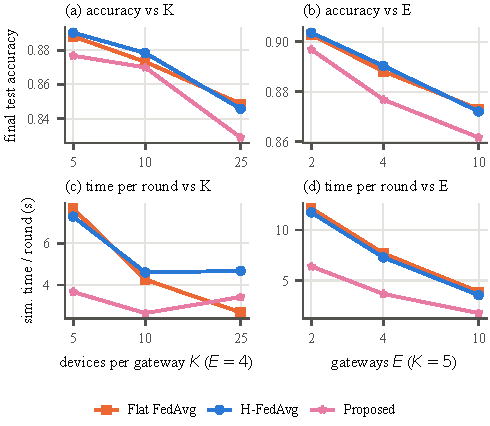
\includegraphics[width=\columnwidth]{figures/fig_rq4_scaling.pdf}}{\figpending{figures/fig\_rq4\_scaling.pdf}}
\caption{RQ4: final accuracy and simulated time per global round as the number of devices per gateway ($K$) and the number of gateways ($E$) grow.}
\label{fig:rq4}
\end{figure}

\subsection{Model Size and Deployment}
The final global model has 80{,}602 parameters and occupies 315~KiB in float32. \todo{int8-quantised size and test-accuracy change after quantisation; inference latency per sample measured on our phones with the benchmark page.}

% ---------------------------------------------------------------------
\section{Discussion and Limitations}
\label{sec:discussion}

\textit{Emulation, not measurement.} The gateways are emulated, and several gateway and network parameters are assumptions (Table~\ref{tab:params}). Absolute times are therefore indicative; the claims of this paper concern relative comparisons between methods under a common, documented cost model.

\textit{Device speeds.} Speed ratios come from published phone measurements and from a browser benchmark on our phones. The browser runtime is not the native on-device training runtime, which is why only ratios are used.

\textit{Model and dataset.} The model is small and Fashion-MNIST is an easy benchmark, so gateway memory and aggregation time are not binding at this scale; the ResNet-18 calculation in Section~\ref{sec:method} shows where they would become binding.

\textit{Simplifications.} Device-to-gateway assignment is static, there is no device mobility or failure other than missed deadlines, links are not contended across gateways, and energy is not modelled.

\todo{One paragraph interpreting the results: what a practitioner deploying Pi-class gateways should take away (e.g., deadline setting, devices per gateway).}

% ---------------------------------------------------------------------
\section{Conclusion and Future Work}
\label{sec:conclusion}

We studied three-tier hierarchical federated learning with heterogeneous devices and resource-constrained, Raspberry Pi-class edge gateways. Using a documented cost model with parameters taken from published measurements and our own phones, we evaluated the cost of heterogeneity, the value of the edge tier, the contribution of FedProx, deadline-based partial aggregation and adaptive local workload, and scaling with the number of devices per gateway. \todo{two or three sentences with the main quantitative findings.}

Future work follows directly from the limitations: (i) replacing the emulated gateways with physical Raspberry Pi boards and measuring aggregation time, memory and energy; (ii) gateway-aware aggregation, such as assigning devices to gateways by capacity or adapting the global synchronisation period $\kappa_2$ to gateway load; (iii) edge-level differential privacy at the gateway; and (iv) harder benchmarks such as CIFAR-10~\cite{krizhevsky2009} and the naturally partitioned FEMNIST~\cite{caldas2018leaf}.

% ---------------------------------------------------------------------
\begin{thebibliography}{99}

\bibitem{mcmahan2017}
H.~B. McMahan, E.~Moore, D.~Ramage, S.~Hampson, and B.~Ag\"{u}era y Arcas, ``Communication-efficient learning of deep networks from decentralized data,'' in \textit{Proc. 20th Int. Conf. Artificial Intelligence and Statistics (AISTATS)}, PMLR, vol.~54, 2017, pp. 1273--1282.

\bibitem{liu2020}
L.~Liu, J.~Zhang, S.~H. Song, and K.~B. Letaief, ``Client-edge-cloud hierarchical federated learning,'' in \textit{Proc. IEEE Int. Conf. Communications (ICC)}, Jun. 2020, pp. 1--6, doi: 10.1109/ICC40277.2020.9148862.

\bibitem{wu2024survey}
J.~Wu, F.~Dong, H.~Leung, Z.~Zhu, J.~Zhou, and S.~Drew, ``Topology-aware federated learning in edge computing: A comprehensive survey,'' \textit{ACM Computing Surveys}, vol.~56, no.~10, pp. 1--41, Oct. 2024, doi: 10.1145/3659205.

\bibitem{bozic2024}
J.~Bo\v{z}i\v{c}, A.~R. Faustino, B.~Radovi\v{c}, M.~Canini, and V.~Pejovi\'{c}, ``Where is the testbed for my federated learning research?,'' in \textit{Proc. IEEE/ACM Symp. Edge Computing (SEC)}, Rome, Italy, Dec. 2024, pp. 249--264, doi: 10.1109/SEC62691.2024.00027.

\bibitem{li2020fedprox}
T.~Li, A.~K. Sahu, M.~Zaheer, M.~Sanjabi, A.~Talwalkar, and V.~Smith, ``Federated optimization in heterogeneous networks,'' in \textit{Proc. Machine Learning and Systems (MLSys)}, vol.~2, 2020, pp. 429--450.

\bibitem{fang2024mtgc}
W.~Fang, D.-J. Han, E.~Chen, S.~Wang, and C.~G. Brinton, ``Hierarchical federated learning with multi-timescale gradient correction,'' in \textit{Advances in Neural Information Processing Systems (NeurIPS)}, vol.~37, 2024, pp. 78863--78904, doi: 10.52202/079017-2504.

\bibitem{luo2024}
L.~Luo, C.~Zhang, H.~Yu, G.~Sun, S.~Luo, and S.~Dustdar, ``Communication-efficient federated learning with adaptive aggregation for heterogeneous client-edge-cloud network,'' \textit{IEEE Trans. Services Computing}, vol.~17, no.~6, pp. 3241--3255, Nov./Dec. 2024, doi: 10.1109/TSC.2024.3399649.

\bibitem{ma2024feduc}
Q.~Ma, Y.~Xu, H.~Xu, J.~Liu, and L.~Huang, ``FedUC: A unified clustering approach for hierarchical federated learning,'' \textit{IEEE Trans. Mobile Computing}, vol.~23, no.~10, pp. 9737--9756, Oct. 2024, doi: 10.1109/TMC.2024.3366947.

\bibitem{woisetschlager2024}
H.~Woisetschl\"{a}ger, A.~Erben, R.~Mayer, S.~Wang, and H.-A. Jacobsen, ``FLEdge: Benchmarking federated learning applications in edge computing systems,'' in \textit{Proc. 25th Int. Middleware Conf. (Middleware)}, Hong Kong, Dec. 2024, pp. 88--102, doi: 10.1145/3652892.3700751.

\bibitem{banerjee2025}
R.~Banerjee \textit{et al.}, ``Flotilla: A scalable, modular and resilient federated learning framework for heterogeneous resources,'' \textit{J. Parallel and Distributed Computing}, vol.~203, Art. no. 105103, Sep. 2025, doi: 10.1016/j.jpdc.2025.105103.

\bibitem{shen2024fedconv}
L.~Shen \textit{et al.}, ``FedConv: A learning-on-model paradigm for heterogeneous federated clients,'' in \textit{Proc. 22nd Annu. Int. Conf. Mobile Systems, Applications and Services (MobiSys)}, Tokyo, Japan, Jun. 2024, pp. 398--411, doi: 10.1145/3643832.3661880.

\bibitem{ma2024esper}
C.~Ma, X.~Li, B.~Huang, G.~Li, and F.~Li, ``Personalized client-edge-cloud hierarchical federated learning in mobile edge computing,'' \textit{J. Cloud Computing}, vol.~13, no.~1, Art. no. 161, 2024, doi: 10.1186/s13677-024-00721-w.

\bibitem{li2024fedcompass}
Z.~Li \textit{et al.}, ``FedCompass: Efficient cross-silo federated learning on heterogeneous client devices using a computing power-aware scheduler,'' in \textit{Proc. Int. Conf. Learning Representations (ICLR)}, 2024. [Online]. Available: \url{https://openreview.net/forum?id=msXxrttLOi}

\bibitem{wu2024fiarse}
F.~Wu, X.~Wang, Y.~Wang, T.~Liu, L.~Su, and J.~Gao, ``FIARSE: Model-heterogeneous federated learning via importance-aware submodel extraction,'' in \textit{Advances in Neural Information Processing Systems (NeurIPS)}, vol.~37, 2024, pp. 115615--115651, doi: 10.52202/079017-3672.

\bibitem{gao2024}
W.~Gao, O.~Tavallaie, S.~Chen, and A.~Zomaya, ``Federated learning as a service for hierarchical edge networks with heterogeneous models,'' in \textit{Service-Oriented Computing (ICSOC 2024)}, Lecture Notes in Computer Science. Singapore: Springer, Dec. 2024, pp. 85--99, doi: 10.1007/978-981-96-0805-8\_6.

\bibitem{wang2023fedch}
Z.~Wang, H.~Xu, J.~Liu, Y.~Xu, H.~Huang, and Y.~Zhao, ``Accelerating federated learning with cluster construction and hierarchical aggregation,'' \textit{IEEE Trans. Mobile Computing}, vol.~22, no.~7, pp. 3805--3822, Jul. 2023, doi: 10.1109/TMC.2022.3147792.

\bibitem{qiu2025}
C.~Qiu, Z.~Wu, H.~Wang, Q.~Yang, Y.~Wang, and C.~Su, ``Hierarchical aggregation for federated learning in heterogeneous IoT scenarios: Enhancing privacy and communication efficiency,'' \textit{Future Internet}, vol.~17, no.~1, Art. no. 18, Jan. 2025, doi: 10.3390/fi17010018.

\bibitem{zhao2024loki}
J.~C. Zhao, A.~Sharma, A.~R. Elkordy, Y.~H. Ezzeldin, S.~Avestimehr, and S.~Bagchi, ``LOKI: Large-scale data reconstruction attack against federated learning through model manipulation,'' in \textit{Proc. IEEE Symp. Security and Privacy (SP)}, May 2024, pp. 1287--1305, doi: 10.1109/SP54263.2024.00030.

\bibitem{su2025}
Y.~Su, W.~Fan, Q.~Meng, P.~Chen, and Y.~Liu, ``Joint adaptive aggregation and resource allocation for hierarchical federated learning systems based on edge-cloud collaboration,'' \textit{IEEE Trans. Cloud Computing}, vol.~13, no.~1, pp. 369--382, Jan. 2025, doi: 10.1109/TCC.2025.3530681.

\bibitem{beutel2020flower}
D.~J. Beutel \textit{et al.}, ``Flower: A friendly federated learning research framework,'' 2020, \textit{arXiv:2007.14390}.

\bibitem{du2025sok}
J.~Du \textit{et al.}, ``SoK: On gradient leakage in federated learning,'' in \textit{Proc. 34th USENIX Security Symp.}, Seattle, WA, USA, Aug. 2025, pp. 3045--3064.

\bibitem{abadi2016}
M.~Abadi, A.~Chu, I.~Goodfellow, H.~B. McMahan, I.~Mironov, K.~Talwar, and L.~Zhang, ``Deep learning with differential privacy,'' in \textit{Proc. ACM SIGSAC Conf. Computer and Communications Security (CCS)}, 2016, pp. 308--318, doi: 10.1145/2976749.2978318.

\bibitem{mcmahan2018dp}
H.~B. McMahan, D.~Ramage, K.~Talwar, and L.~Zhang, ``Learning differentially private recurrent language models,'' in \textit{Proc. Int. Conf. Learning Representations (ICLR)}, 2018.

\bibitem{bonawitz2017}
K.~Bonawitz \textit{et al.}, ``Practical secure aggregation for privacy-preserving machine learning,'' in \textit{Proc. ACM SIGSAC Conf. Computer and Communications Security (CCS)}, 2017, pp. 1175--1191, doi: 10.1145/3133956.3133982.

\bibitem{xiao2017fmnist}
H.~Xiao, K.~Rasul, and R.~Vollgraf, ``Fashion-MNIST: A novel image dataset for benchmarking machine learning algorithms,'' 2017, \textit{arXiv:1708.07747}.

\bibitem{hsu2019}
T.-M.~H. Hsu, H.~Qi, and M.~Brown, ``Measuring the effects of non-identical data distribution for federated visual classification,'' 2019, \textit{arXiv:1909.06335}.

\bibitem{smilkov2019tfjs}
D.~Smilkov \textit{et al.}, ``TensorFlow.js: Machine learning for the web and beyond,'' in \textit{Proc. Machine Learning and Systems (MLSys)}, vol.~1, 2019, pp. 309--321.

\bibitem{rpi4brief}
Raspberry Pi Ltd., ``Raspberry Pi 4 Model B product brief,'' 2019. [Online]. Available: \url{https://datasheets.raspberrypi.com/rpi4/raspberry-pi-4-product-brief.pdf}

\bibitem{he2016resnet}
K.~He, X.~Zhang, S.~Ren, and J.~Sun, ``Deep residual learning for image recognition,'' in \textit{Proc. IEEE Conf. Computer Vision and Pattern Recognition (CVPR)}, 2016, pp. 770--778.

\bibitem{paszke2019pytorch}
A.~Paszke \textit{et al.}, ``PyTorch: An imperative style, high-performance deep learning library,'' in \textit{Advances in Neural Information Processing Systems (NeurIPS)}, vol.~32, 2019, pp. 8024--8035.

\bibitem{krizhevsky2009}
A.~Krizhevsky, ``Learning multiple layers of features from tiny images,'' Univ. of Toronto, Tech. Rep., 2009.

\bibitem{caldas2018leaf}
S.~Caldas \textit{et al.}, ``LEAF: A benchmark for federated settings,'' 2018, \textit{arXiv:1812.01097}.

\end{thebibliography}

\end{document}
